% Number 200
% CVPMG Units
% v to x graph, quantitative
% Walker

% Watermark
\AddToShipoutPicture*{\BackgroundPic}

\addtocounter {ProbNum} {1}

%\begin{floatingfigure}[r]{.3\textwidth}
%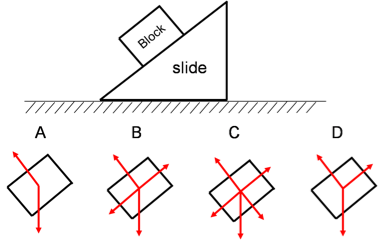
\includegraphics[scale=.4]{/Users/jgates/desktop/latex/pics/incline3.png}
%\end{floatingfigure}
 
{\bf \Large{\arabic{ProbNum}}} Construct a position-vs-time graph for the motion described in the v vs t graph shown below. Assume a position of 10 meters at t = 0. Be sure to number the scale on the position axis.. 

\bigskip

%What was your original speed?  
\begin{center}
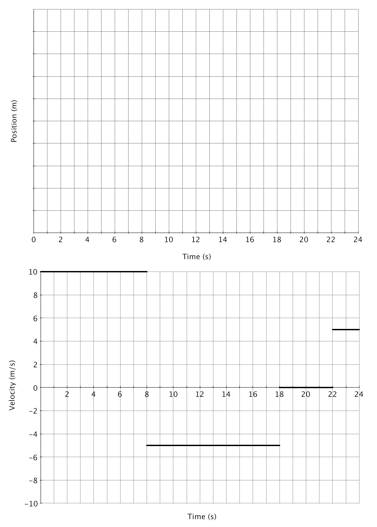
\includegraphics[scale=.77]{/Users/jgates/desktop/latex/pics/vtoxgraph1.png}
\end{center}

\vfill

\newpage